\section{The Definite Integral}

For reasons that will not be immediately obvious, integration is opposite differentiation on the `calculus coin.'

\subsection{The Definite Integral}

The \textbf{definite integral of $f$ on $(a,b)$} is written 
$$\int_a^bf(x)\ dx$$
and is defined to be the \textit{signed} area between the graph of $f$ and the $x$-axis (if such a quantity exists). \mar{When might this quantity not exist?}

\begin{figure}[h!]
\centering
\fbox{
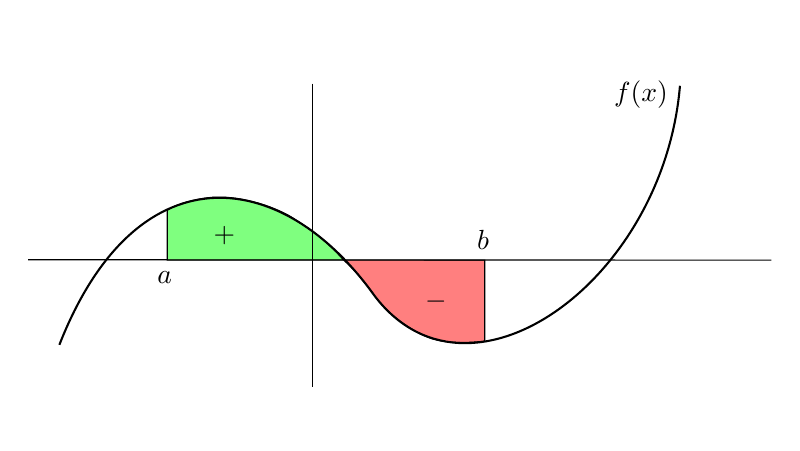
\begin{tikzpicture}[x=0.75pt,y=0.75pt,yscale=-1,xscale=1]
\path (150,50);

%Shape: Polygon Curved [id:ds707129257032501] 
\draw  [fill={rgb, 255:red, 0; green, 255; blue, 0 }  ,fill opacity=0.5 ] (217,162) .. controls (217,162) and (217,138) .. (217,138) .. controls (217,138) and (222,134) .. (236,132) .. controls (250,130) and (269,136) .. (278,142) .. controls (287,148) and (288.41,149.01) .. (293,153) .. controls (297.59,156.99) and (302,162) .. (302,162) .. controls (302,162) and (217,162) .. (217,162) -- cycle ;
%Shape: Polygon Curved [id:ds12696670726714787] 
\draw  [fill={rgb, 255:red, 255; green, 0; blue, 0 }  ,fill opacity=0.5 ] (370,162) .. controls (370,162) and (370,201) .. (370,201) .. controls (370,201) and (355,203) .. (345,200) .. controls (335,197) and (322,187) .. (316,178) .. controls (310,169) and (302,162) .. (302,162) .. controls (302,162) and (370,162) .. (370,162) -- cycle ;
%Straight Lines [id:da2259128899132099] 
\draw    (150,161.8) -- (508,162) ;
%Straight Lines [id:da519801972092973] 
\draw    (287,77) -- (287,223) ;
%Curve Lines [id:da2537963372820191] 
\draw [line width=0.75]    (165,202.8) .. controls (201.6,109.5) and (271,116) .. (316,178) .. controls (361,240) and (456,173) .. (464,78) ;
%Straight Lines [id:da8858936847665124] 
\draw    (217,138) -- (217,162) ;
%Straight Lines [id:da05784827822991523] 
\draw    (370,162) -- (370,201) ;

% Text Node
\draw (211,166.4) node [anchor=north west][inner sep=0.75pt]    {$a$};
% Text Node
\draw (365,146.4) node [anchor=north west][inner sep=0.75pt]    {$b$};
% Text Node
\draw (431,74.4) node [anchor=north west][inner sep=0.75pt]    {$f( x)$};
% Text Node
\draw (238,144.4) node [anchor=north west][inner sep=0.75pt]    {$+$};
% Text Node
\draw (340,176.4) node [anchor=north west][inner sep=0.75pt]    {$-$};
\end{tikzpicture}
}

\caption{The Geometric Definition of the Definite Integral}
\end{figure}


The figure shows the meaning of the word ``signed'': areas that are above the $x$-axis are counted as positive, while those below are negative.

With no other tools available to you, the only way to compute definite integrals right now is to draw the graph of $f$ and compute the desired area using your knowledge of geometry. \mar{Compute $$\int_{-3}^72x+4\ dx$$ using geometry.} This can be easy if $f$ is made up of lines and circular arcs, but if not, the way to compute a definite integral is not immediately obvious.

\subsection{Reimann Sums}

The first way that we will attempt to compute definite integrals is with a limit of a Riemann sum. We will start by approximating the area by a collection of vertical rectangles. Refer to the figure as an example as we construct a Riemann sum.

\begin{figure}[h!]
\centering
\fbox{    


\tikzset{every picture/.style={line width=0.75pt}} %set default line width to 0.75pt        

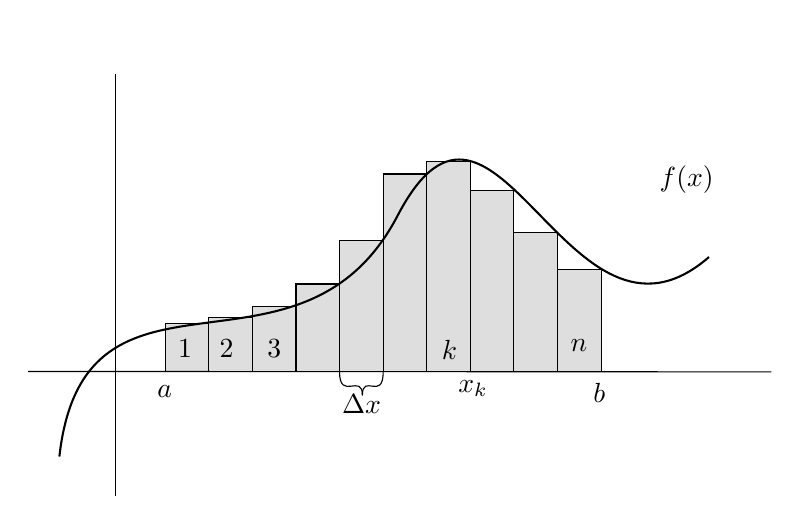
\begin{tikzpicture}[x=0.75pt,y=0.75pt,yscale=-1,xscale=1]
%uncomment if require: \path (0,300); %set diagram left start at 0, and has height of 300

%Shape: Rectangle [id:dp7232780056512873] 
\draw  [fill={rgb, 255:red, 222; green, 222; blue, 222 }  ,fill opacity=1 ] (217,145.67) -- (238,145.67) -- (238,169) -- (217,169) -- cycle ;
%Shape: Rectangle [id:dp9564785112393279] 
\draw  [fill={rgb, 255:red, 222; green, 222; blue, 222 }  ,fill opacity=1 ] (238,142.67) -- (259,142.67) -- (259,169) -- (238,169) -- cycle ;
%Shape: Rectangle [id:dp3339762801991184] 
\draw  [fill={rgb, 255:red, 222; green, 222; blue, 222 }  ,fill opacity=1 ] (259,137.67) -- (280,137.67) -- (280,169) -- (259,169) -- cycle ;
%Shape: Rectangle [id:dp8735502353012137] 
\draw  [fill={rgb, 255:red, 222; green, 222; blue, 222 }  ,fill opacity=1 ] (280,126.67) -- (301,126.67) -- (301,169) -- (280,169) -- cycle ;
%Shape: Rectangle [id:dp9736947359557422] 
\draw  [fill={rgb, 255:red, 222; green, 222; blue, 222 }  ,fill opacity=1 ] (301,105.67) -- (322,105.67) -- (322,169) -- (301,169) -- cycle ;
%Shape: Rectangle [id:dp462370433249887] 
\draw  [fill={rgb, 255:red, 222; green, 222; blue, 222 }  ,fill opacity=1 ] (322,73.67) -- (343,73.67) -- (343,169) -- (322,169) -- cycle ;
%Shape: Rectangle [id:dp30050179546388955] 
\draw  [fill={rgb, 255:red, 222; green, 222; blue, 222 }  ,fill opacity=1 ] (343,67.67) -- (364,67.67) -- (364,169) -- (343,169) -- cycle ;
%Shape: Rectangle [id:dp5888931362167766] 
\draw  [fill={rgb, 255:red, 222; green, 222; blue, 222 }  ,fill opacity=1 ] (364,81.67) -- (385,81.67) -- (385,169) -- (364,169) -- cycle ;
%Shape: Rectangle [id:dp23162244325779224] 
\draw  [fill={rgb, 255:red, 222; green, 222; blue, 222 }  ,fill opacity=1 ] (385,101.67) -- (406,101.67) -- (406,169) -- (385,169) -- cycle ;
%Shape: Rectangle [id:dp5505196011593232] 
\draw  [fill={rgb, 255:red, 222; green, 222; blue, 222 }  ,fill opacity=1 ] (406,119.67) -- (427,119.67) -- (427,169) -- (406,169) -- cycle ;
%Straight Lines [id:da015408719112721014] 
\draw    (151,168.8) -- (509,169) ;
%Straight Lines [id:da7870970100056962] 
\draw    (193,25.67) -- (193,229) ;
%Curve Lines [id:da23517536685350726] 
\draw [line width=0.75]    (166,209.8) .. controls (178,103.67) and (282,183.67) .. (329,93.67) .. controls (376,3.67) and (411,172.67) .. (479,113.67) ;
%Curve Lines [id:da8766831258062089] 
\draw    (301,169) .. controls (301,183.33) and (312,169.33) .. (312,180.33) ;
%Curve Lines [id:da8471782229516964] 
\draw    (322,169) .. controls (322,183.33) and (312,169.33) .. (312,180.33) ;

% Text Node
\draw (212,174.4) node [anchor=north west][inner sep=0.75pt]    {$a$};
% Text Node
\draw (422,173.4) node [anchor=north west][inner sep=0.75pt]    {$b$};
% Text Node
\draw (454,68.4) node [anchor=north west][inner sep=0.75pt]    {$f( x)$};
% Text Node
\draw (222,152.4) node [anchor=north west][inner sep=0.75pt]    {$1$};
% Text Node
\draw (242,152.4) node [anchor=north west][inner sep=0.75pt]    {$2$};
% Text Node
\draw (265,152.4) node [anchor=north west][inner sep=0.75pt]    {$3$};
% Text Node
\draw (411,152.4) node [anchor=north west][inner sep=0.75pt]    {$n$};
% Text Node
\draw (349,152.4) node [anchor=north west][inner sep=0.75pt]    {$k$};
% Text Node
\draw (301,178.73) node [anchor=north west][inner sep=0.75pt]    {$\Delta x$};
% Text Node
\draw (357,171.73) node [anchor=north west][inner sep=0.75pt]    {$x_{k}$};


\end{tikzpicture}

}
\caption{A Right Reimann Sum}
\end{figure}

Divide the interval $(a,b)$ into $n$ equal sub-intervals, each with width $\Delta x= \frac{b-a}{n}$. Then for each sub-interval draw a rectangle with base length $\Delta x$ on the $x$-axis and height determined by the value of $f$ at the right endpoint of the sub-interval. The right endpoint of the $i$th sub-interval is $x_k=a+k\Delta x$, so the area of the $k$th rectangle is $f(x_k) \Delta x$. The area of all $n$ rectangles together is
$$\sum_{k=1}^{n}f(x_k)\Delta x.$$
Since we used the \textit{right} endpoint of each sub-interval, we call this quantity the \textbf{$n$th Right Riemann Sum}:
$$R_n=\sum_{k=1}^{n}f\left(a+k\frac{b-a}{n}\right)\frac{b-a}{n}.$$
We could also have used the \textit{left} endpoint of each sub-interval to determine the height of each box, in which case we would get the \textbf{$n$th Left Riemann Sum}:\mar{Draw a picture of $L_n$.}
$$L_n=\sum_{k=1}^{n}f\left(a+(k-1)\frac{b-a}{n}\right)\frac{b-a}{n}.$$
If instead we use trapezoids above each sub-interval, we get the \textbf{$n$th Trapezoid Riemann Sum}: \mar{Draw a picture of $T_n$.}
$$T_n=\sum_{i=k}^{n}\frac{f\left(a+(k-1)\frac{b-a}{n}\right)+f\left(a+k\frac{b-a}{n}\right)}{2}\frac{b-a}{n}=\frac{R_n+L_n}{2},$$
where the $k$th trapezoid has width $\Delta x$ and heights determined by the left and right endpoints of the $k$th sub-interval. (Remember that a trapezoid with width $w$ and heights $h_1$ and $h_2$ has area $A=\frac{h_1+h_2}{2}w$. \mar{When are $R_n$, $L_n$, and $T_n$ overestimates? Underestimates?}

In practice, it doesn't matter which you choose to compute because of the following theorem:
\begin{thm} With the notation as above,
$$\lim_{n\to\infty}R_n=\lim_{n\to\infty}L_n=\lim_{n\to\infty}T_n=\int_a^bf(x)\ dx.$$
\end{thm}

This theorem should be intuitive: as $n$ gets larger, the width of each rectangle gets smaller and the approximation gets better.

For large $n$, a Riemann sum can give a very good approximation, but in general it is not feasible to do by hand. However, if $f$ is a polynomial it is not hard to compute $R_n$ algebraically and then take a limit. In order to do so, we'll need the following summation identities:
\begin{align*}
&\sum_{k=1}^n 1 = n 
& &
\sum_{k=1}^n k = \frac{n(n+1)}{2}\\
&\sum_{k=1}^n k^2 = \frac{n(n+1)(2n+1)}{6}
& &
\sum_{k=1}^n k^3 = \frac{n^2(n+1)^2}{4}
\end{align*}

Here is an example:
\begin{itemize}
    \item To compute $\int_{0}^{1}x^2+x\ dx$, first find $R_n$:
    \begin{align*}
        R_n
        & = \sum_{k=1}^{n}f\left(a+k\frac{b-a}{n}\right)\frac{b-a}{n}\\ 
        & = \sum_{k=1}^n\left(\left(0+k\frac{1-0}{n}\right)^2 + \left(0+k\frac{1-0}{n}\right)\right)\frac{1-0}{n}&&&\text{plug in}\\
        & = \sum_{k=1}^n\left(\frac{k^2}{n^2} + \frac{k}{n}\right)\frac{1}{n} &&&\text{expand and simplify}\\
        & = \frac{1}{n^3}\sum_{k=1}^nk^2+\frac{1}{n^2}\sum_{k=1}^nk &&& \text{factor}\\
        & = \frac{1}{n^3}\frac{n(n+1)(2n+1)}{6}+\frac{1}{n^2}\frac{n(n+1)}{2} &&&\text{use sum identities}
    \end{align*}
    Then take the limit:
    $$\lim_{n\to\infty}R_n=\lim_{n\to\infty} \frac{1}{n^3}\frac{n(n+1)(2n+1)}{6}+\frac{1}{n^2}\frac{n(n+1)}{2} = \frac{2}{6} + \frac{1}{2} = \frac{5}{6}.$$
    
\end{itemize}

\mar{Compute $$\int_{0}^1x^3\ dx$$ using the method of Riemann Sums.}


\subsection{The Fundamental Theorem of Calculus}

Let's cut right to the chase:

\begin{thm}[The Fundamental Theorem of Calculus]
    $$\int_a^bf(x)\ dx = F(b)-F(a),$$
    where $F'=f$.
\end{thm}

This theorem is the connection between differentiation and integration! It is also how we will compute definite integrals from now on:
\begin{enumerate}
    \item Find a function $F$ for which $F'=f$.
    \item Evaluate $F(b)-F(a).$
\end{enumerate}

The first point is called \textbf{anti-differentiation}, and is the harder step. Before we get to that, let's try to understand how this theorem agrees with our intuition about Riemann Sums. If we take the $b$-derivative of the equation in the theorem, we get
$$\frac{d}{db}\left[\int_a^{b}f(x)\ dx\right] = \frac{d}{db}\left[F(b)-F(a)\right] = f(b).$$
This means that the rate at which the area is changing is $f(b)$. This makes sense in terms of Riemann sums: if we increase $b$ by a small amount $\Delta b$, the area will change by about $f(b) \Delta b$. Thus the derivative of the area is $f(b)\Delta b/\Delta b = f(b)$. \mar{Draw a picture of $b$ increasing by $\Delta b$. Then sit and really think about this until it makes sense.}













